
\section{Entwicklung einer Handlungsempfehlung}
\label{sec:Handlungsempfehlung}
Um in einem von intensivem Wettbewerb geprägten Geschäftsumfeld zu bestehen, ist es für Unternehmen von entscheidender Bedeutung, effiziente und agile Bereitstellungsverfahren zu implementieren. Infolgedessen verwenden 62 Prozent aller Unternehmensentwickler CI/CD-Tools innerhalb ihrer Bereitstellungsprozesse. Das CI/CD-Verfahren bietet dabei insbesondere für CEs erhebliche Vorteile. Obwohl einzelne Module einer CEA grundsätzlich isoliert voneinander betrieben werden, können über Schnittstellen Abhängigkeiten entstehen. Insbesondere bei der Zusammenarbeit vieler Entwickler kann die Implementierung und Integration neuer IT-Services deshalb zu erheblichem Koordinationsaufwand führen. Wenn Teams nicht in der Lage sind, effektiv miteinander zu kommunizieren, besteht das Risiko, dass Konflikte in der gemeinsamen Code-Basis entstehen. Um dieser Herausforderung zu begegnen, empfiehlt sich eine Automatisierung korrespondierender CI-Prozesse. Dabei wird der lokale Quellcode der Entwickler kontinuierlich und automatisiert mit dem Hauptzweig des Repositories zusammengeführt und mit dem bestehenden Code getestet. Statt Code-Reviews und Validierungen erst in einer späten Phase des Softwareerstellungszykluses abzuwickeln (\textit{Shift-Right}), ermöglicht die CI/CD-Pipeline, dass Tests bereits während der Entwicklung durchgeführt werden (\textit{Shift-Left}). Somit erlangen Entwickler kontinuierliches Feedback und können Services optimieren, bis diese den Produktstandards des Unternehmens entsprechen. Darüber hinaus ermöglichen CI/CD-Pipelines den Aufbau standardisierter Testinfrastrukturen. Damit können neue Features automatisiert in Systemumgebungen getestet werden, bei welchen Betriebssysteme, Systembibliotheken, Abhängigkeiten und Konfigurationseinstellungen an die Produktion angepasst sind. Zum einen können so potenzielle, im Produktionssystem auftretende Fehlerquellen erkannt werden. Darüber hinaus entfällt durch das automatische Abwickeln dieser Prozesse ein manuelles Aufsetzen der Testinfrastruktur, wobei CEs ihre IT-Ressourcen verstärkt auf Entwicklung neuer Services fokussieren können.\\ Damit Unternehmen schnell von diesen Diensten profitieren können, ist es von essenzieller Bedeutung, dass nicht nur das Testen, sondern ebenfalls die Bereitstellung neuer IT-Services kontinuierlich und automatisiert abgewickelt wird. Durch das unmittelbare Kompilieren, Validieren und Versionieren bei der Integration neuen Codes, steht zu jedem Zeitpunkt eine für die Veröffentlichung geeignete Anwendungsversion im zentralen Repository bereit. Unter Zuhilfenahme eines effektiven CD-Prozesses kann somit ein mehrfaches tägliches Ausrollen der Dienste ermöglicht werden. Dies führt zur Verkürzung des \textit{Time-To-Values}, also dem Zeitintervall, bis der entwickelte IT-Service den ersten Kundennutzen herbeiführt \cite{Prof.Dr.RalfT.Kreutzer.20180215}. Anstelle der Bereitstellung einer vollständig implementierten Anwendung bezweckt das CI/CD-Verfahren ein inkrementelles und frühes Ausrollen kleiner Features. Zwar besteht hierbei das Risiko, dass der Kundennutzen im Vergleich zur Kompletteinführung zunächst abgeschwächt ist, jedoch ermöglicht diese Früheinführung eine zügige Akkumulation und Umsetzung des Anwenderfeedbacks \cite[9]{Halstenberg.2020}.\\ 
Entschließt sich ein CE dazu, Bereitstellungsprozesse zu automatisieren, sollte dieses strategisch vorgehen. So empfiehlt Experte 5, Softwarearchitekt des SAP DTS, ein schrittweises Implementieren der Pipeline. Dabei sollte zunächst Erfahrung mit der Automatisierung einfacher isolierter Prozesse gesammelt werden \cite[Z. 8 ff.]{SoftwareArchitektSAPDTSIntegration.}. Anschließend können verbleibende, zur Bereitstellung von Software benötigten Schritte, in einem kontrollierten Tempo in die Pipeline eingebunden werden. Bei der Einführung von CI/CD ist dabei ebenso entscheidend, dass Unternehmen spezifische Anforderungen abdeckende Tools verwenden. Dafür wurde im Rahmen dieser Arbeit ein Entscheidungs-Framework entworfen. Mit diesem wurde evaluiert, welches Pipeline-Tool zur Automatisierung der CI/CD-Prozesse für eine CEA den größten Mehrwert birgt.\\ Unter Berücksichtigung der in Kapitel \ref{sec:Bewertung} abgewickelten Analyse, kann Azure Pipelines als das optimale CI/CD-Tool angesehen werden. Aus diesem Kontext lassen sich für das Pipeline-Tool einige Vorteile ableiten. Azure Pipelines unterstützt die Programmbibliothek Project Piper, mit welcher essenzielle Schritte für das Bauen, Testen und Bereitstellen von SAP-CAP-Node- und SAP-UI5-Anwendungen ausgeliefert werden. Die Programmbibliothek gewährleistet, dass sämtliche Compliance-Standards der SAP, wie Sicherheits- und Datenschutzbestimmungen, Branchenvorschriften oder interne Richtlinien bei der Entwicklung von IT-Services eingehalten werden. Obwohl die vorliegende Arbeit zur Beratung externer Kunden konzipiert ist, welche nicht verpflichtet sind, diese Richtlinien einzuhalten, sind diese oft in kritischen Sektoren tätig, bei welchen ebenfalls strikte Regularien gelten. Durch die Bereitstellung dieser standardisierten Bibliothek entfällt für Unternehmensentwickler somit die Notwendigkeit einer zeitaufwendigen Implementierung dieser Schritte.\\ Darüber hinaus werden für Azure Pipelines umfassende Bereitstellungsfunktionalitäten ausgeliefert. Dazu gehört das Blue/Green-Deployment. Dieses stellt eine effektive Möglichkeit dar, Software unter Produktionsbedingungen zu testen und kritische Ausfallzeiten bei der Bereitstellung von Software zu vermeiden. Dies spielt insbesondere eine wichtige Rolle, wenn Fehler in einem Service eines ERP-Systems auftreten, jedoch das herkömmliche Bereitstellen einer neuen Anwendungsversion aufgrund der durch die Initialisierung  bedingten Ausfallzeit, zu unflexibel ist. Ein weiteres mit Azure Pipelines kompatibles Bereitstellungskonzept ist das Multi-Cloud-Deployment. Mit diesem können einzelne Module auf unterschiedlichen Cloud-Plattformen ausgerollt werden. Neben einer Bereitstellung auf etablierten Cloud-Plattformen wie Google Cloud oder Amazon Web Services ermöglicht Azure Pipelines in diesem Kontext ebenfalls eine nahtlose Integration mit der eigenen Cloud-Plattform.\\
Dieser Integrationsvorteil erstreckt sich ebenfalls auf andere Services, welche innerhalb des Azure-Ökosystems bereitgestellt werden. Dazu gehören Produkte wie eine Entwicklungsumgebung, ein Projektmanagement- und Monitoring-Tool sowie ein Artefakt-Repository. Durch die Verwendung dieser Integrationsmöglichkeiten kann eine Rationalisierung des Entwicklungsprozesses erreicht werden. So ist es Entwicklern etwa möglich, Tests der Integration-Pipeline unmittelbar aus der Visual-Studio-Code-Umgebung auszuführen oder den Build-Status verschiedener Pipelines in einem zentralen Monitoring-Tool zu überwachen. Eine weitere Rationalisierung des Bereitstellungsprozesses kann durch die Verwendung verschiedener Ausführungs\-mechanismen erzielt werden. Im Falle von Fehlschlägen einzelner Schritte, besteht die Möglichkeit, dass nur fehlerhafte Schritte erneut ausgeführt werden. Auf diese Weise lassen sich bei temporären Problemen oder externen Abhängigkeiten, wie Ausfällen von Drittanbietern, Zeit und Rechenressourcen einsparen.\\ Dies erwies sich ebenfalls im One-Strike-Programm als einen bedeutenden Aspekt. In dem One-Strike-Programm hat die SAP Maßnahmen ergriffen, um die Anzahl der Cloud-Provider, von welchen Dienste bezogen werden, zu reduzieren. Im Rahmen dieser Konsolidierung wurden Frontend-End-Pipelines für das S/4HANA-Core, welche zuvor auf Jenkins gehostet wurden, zu Azure migriert. In diesem Zusammenhang waren ebenfalls Kostenüberlegungen ein ausschlaggebender Aspekt für den Wechsel auf Azure. Durch die Nutzung einer SaaS-basierten CI/CD-Lösung können erhebliche Einsparungen bei Aufwandspositionen wie Hardwareinvestitionen oder Wartungs- und Support-Kosten erzielt werden. Dieser Aspekt birgt insbesondere einen erheblichen Mehrwert für die CEA. Da Unternehmen mit dieser Architektur bestrebt sind, schnell auf disruptive Marktveränderungen zu reagieren, müssen CEs in der Lage sein, Services wie CI/CD-Pipelines schnell auf- und abbauen bzw. skalieren zu können. Während in einem On-Premise-Modell hierfür ggf. hohe Investitionen erforderlich sind, werden Rechenressourcen bei Azure unmittelbar bereitgestellt und in Abhängigkeit der Nutzung bepreist (\textit{Pay-as-you-go}).\\ Da die Bereitstellung von Services zum Kerngeschäft von Microsoft gehört, wird kontinuierlich in die Aktualisierung und Verbesserung der Azure-Infrastruktur investiert. Neben der Verwendung neuester Hardware wird die hohe Leistungsfähigkeit von Azure Pipelines ebenfalls durch das Bereitstellen von Optimierungsmechanismen sichergestellt. Dazu gehört etwa das parallele Ausführen verschiedener Pipeline-Schritte oder die Verwendung von Caching. Laut Experte 4 haben diese Konzepte dazu beitragen, dass der CI/CD-Prozess der SAP-Standardentwicklung um 35 Prozent beschleunigt wurde \cite[Z. 58 ff.]{TestDeveloperSAPHyperspaceAdoption&Onboarding.}.\\ Obwohl Azure Pipelines die für eine CEA essenziellen Funktionalitäten bereitstellt, besteht die Möglichkeit, dass Unternehmen aufgrund situativer Gegebenheiten, stattdessen Jenkins oder SAP CI/CD verwenden sollten. Dafür ausschlaggebende Gründe werden in dem folgenden Entscheidungsbaum aufgeführt:
\begin{center}
	\begin{figure}[H]\hspace*{-11mm}
		\centering
		\scalebox{0.5}{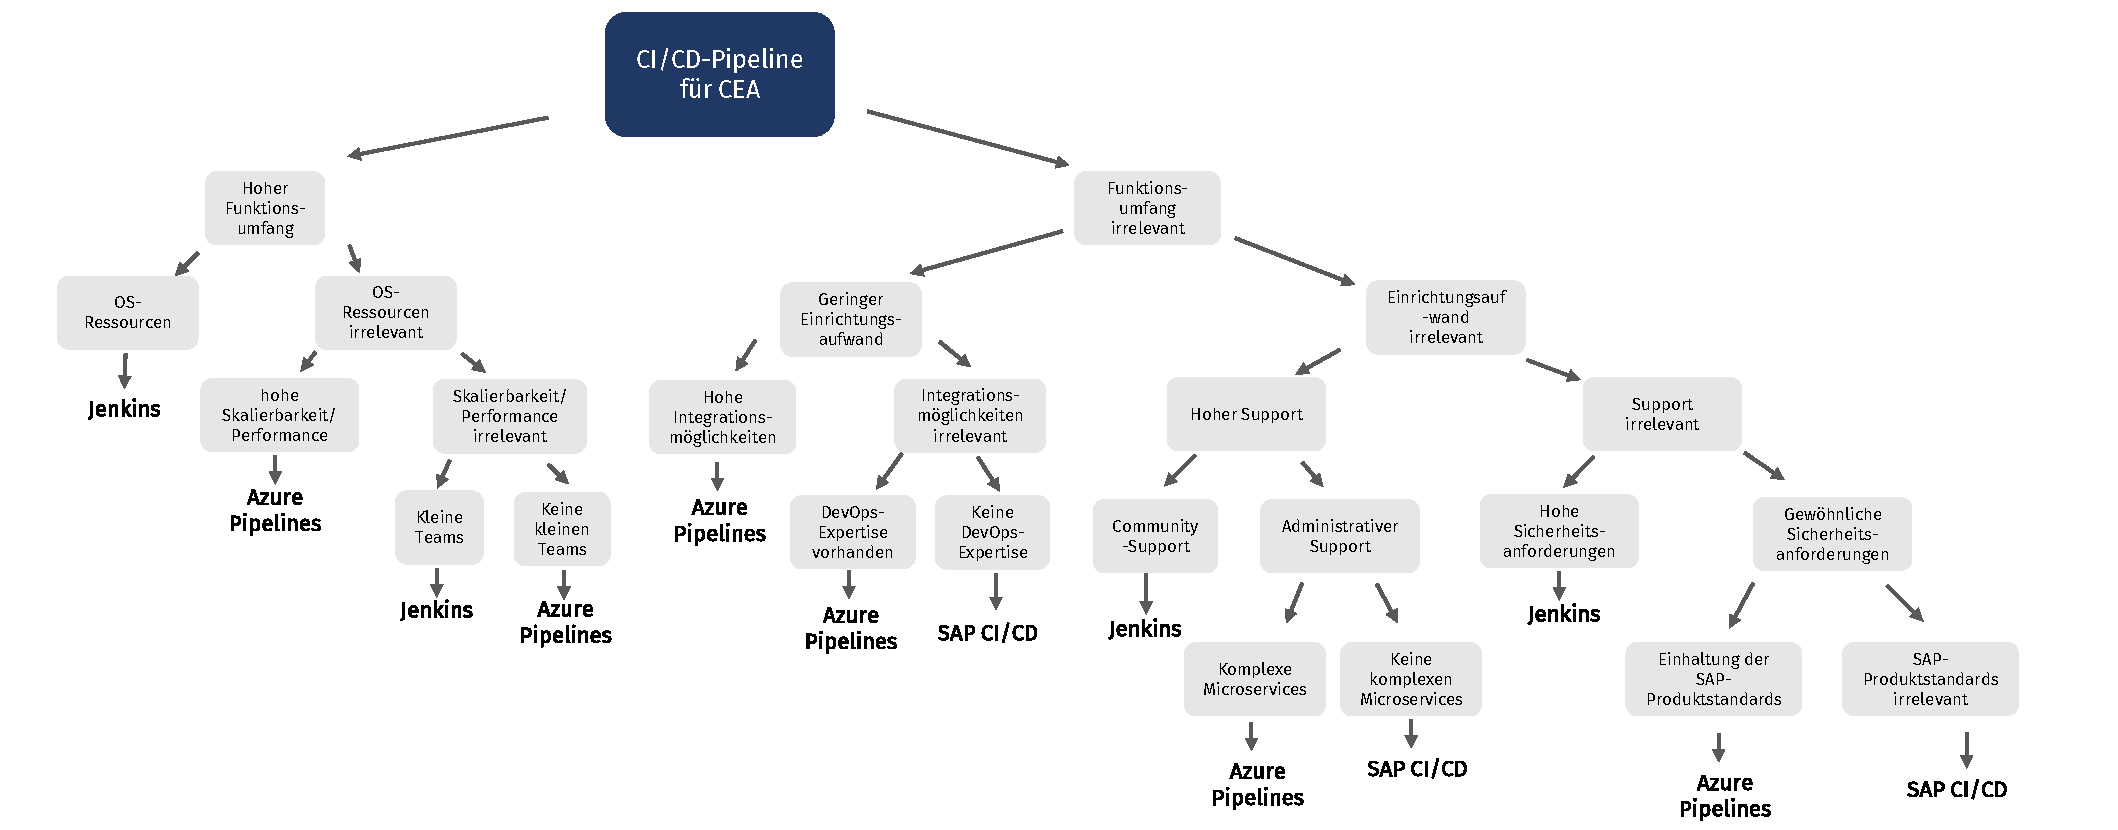
\includegraphics{Entscheidungsbaum}}
		\caption[Entscheidungsbaum für die Wahl eines CI/CD-Pipeline-Tools]{Entscheidungsbaum für die Wahl eines CI/CD-Pipeline-Tools. Eigene Darstellung.}
		\label{fig:Entscheidungsbaum}
	\end{figure}
\end{center}
\vspace*{-15mm}
Laut Experte 1 sollte SAP CI/CD insbesondere von Kunden verwendet werden, welche über eine geringe Anzahl an Microservices verfügen und somit keine komplexen Anforderungen an den Bereitstellungsprozess besitzen \cite[Z. 58 ff.]{ProductOwnerSAPBTPProd&Infra.}. Auch wenn mit SAP CI/CD für SAP CAP Node sowie SAP UI5 essenzielle Pipeline-Schritte bereitgestellt werden, sind Unternehmen mit diesem Tool in ihren Funktionalitäten eingeschränkt. Dies ist maßgeblich darauf zurückzuführen, dass das CI/CD-Tool ausschließlich eine Konfiguration und keine Implementierung der Pipelines zulässt. 
Laut Experte 1 ist dieses Tool jedoch insbesondere für Kunden vorgesehen, welche aus der traditionellen On-Premise-Umgebung auf die SAP BTP umsteigen \cite[Z. 58 ff.]{ProductOwnerSAPBTPProd&Infra.}. Hierbei besitzen Entwicklungsteams i.d.R. nicht über erforderliche DevOps-Kenntnisse, da diese zunächst mit dem Lernen allgemeiner Cloud-Konzepte, wie z.B. Programmier-Frameworks, beschäftigt sind. So soll das im Jahr 2020 veröffentlichte Tool kontinuierlich erweitert werden, um den wachsenden Anforderungen der Nutzer gerecht zu werden. 
Weiterhin empfiehlt sich dieses Tool für CEs, welche bereits ein umfangreiches Produktportfolio der SAP beziehen und auch zukünftig auf SAP-Technologien setzen möchten. So könnten SAP-Kunden, welche neben SAP CI/CD ebenfalls andere Services des Unternehmens beziehen, potenziell von niedrigeren Gebühren für das Tool profitieren.\\ Eine weitaus höhere Flexibilität ergibt sich durch die Verwendung von Jenkins. Da dieses CI/CD-Tool On-Premise bereitgestellt wird, besitzt ein Unternehmen volle Kontrolle über die Gestaltung des Pipeline-Tools und kann dieses somit auf die Bedürfnisse der eigenen Systemarchitektur ausrichten. Dies ermöglicht eine flexible Anpassung der Infrastrukturkomponenten, wie Server- und Netzwerkmodule, Sicherheitsprotokolle oder dem Datenmanagement. Somit bietet sich eine On-Premise-Pipeline insbesondere in Branchen an, in welchen Datensicherheit und Compliance-Anforderungen hohe Priorität besitzen. Ein zusätzliches Argument für den Einsatz von Jenkins ist die Unabhängigkeit von den im Standard bereitgestellten Funktionalitäten. Durch den Open-Source-Charakter des Tools stehen den Entwicklern zahlreiche externe Ressourcen zur Verfügung. Dies können etwa von der Community entwickelte Plug-ins darstellen, welche in das Pipeline-System integriert werden können. Darüber hinaus haben DevOps-Spezialisten Zugang auf eine Vielzahl in Internetforen veröffentlichte Informationen. Dies unterstützt Entwickler dabei, Expertise, welche zur Implementierung einer maßgeschneiderten Pipeline benötigt wird, zu erlangen. Experte 4 bemerkt, dass Jenkins jedoch ausschließlich von kleinen Entwicklungsteams, welche mit einer geringen Anzahl an Technologien arbeiten, verwendet werden sollte \cite[Z. 58 ff.]{TestDeveloperSAPHyperspaceAdoption&Onboarding.}. Dies lässt sich darauf zurückführen, dass durch eine Aktualisierung diverse Plug-ins mit der neuen Jenkins-Version inkompatibel sein könnten. Folglich tendieren große Entwicklungsprojekte, welche eine Vielzahl heterogener Plug-ins verwenden, dazu, eine Aktualisierung hinauszuzögern. Dies kann dazu führen, dass potenzielle Sicherheitslücken und Fehler des Jenkins-Systems nicht behoben werden können. Somit sollte darauf geachtet werden, dass dieses Pipeline-System ausschließlich in kleinen Entwicklungsprojekten mit wenig Abhängigkeiten verwendet wird.  
